% !TEX root = /doc.tex

\section{Methodology}

\subsection{Creation of Dataset}

The data set forms the basis for the training of the Machine Learning Classifiers and is created specifically for this work using commit data from 13 feature-based software projects. The software projects are selected based on previous use in scientific literature \cite{Hunsen2015,Liebig2010,Queiroz2015,Queiroz2016}. However, it was also important that the variability in the source code of the software projects was implemented by means of preprocessor directives and that their git repositories had a clear "revision history" regarding release numbers. Another sufficient criterion was the use of a common language. All software projects originate from the English-speaking world. The software projects used for this work are listed in \autoref{tab:tools} together with their purpose and data sources.

\begin{table}[ht]
\centering
\caption{Used software projects}
\label{tab:tools}
\resizebox{\linewidth}{!}{%
\begin{tabular}{|l|l|l|} 
\hline
 \textbf{Project}  & \textbf{Purpose}  & \textbf{Data source}    \\ 
\hline
\textbf{Blender}   & 3D modelling tool & GitHub mirror           \\ 
\hline
\textbf{Busybox}   & UNIX toolkit      & Git repository          \\ 
\hline
\textbf{Emacs}     & text editor       & GitHub mirror           \\ 
\hline
\textbf{GIMP}      & graphics editor   & GitLab repository       \\ 
\hline
\textbf{Gnumeric}  & spreadsheet       & GitLab repository       \\ 
\hline
\textbf{gnuplot}   & plotting tool     & GitHub mirror           \\ 
\hline
\textbf{Irssi}     & IRC client        & GitHub repository       \\ 
\hline
\textbf{libxml2}   & XML parser        & GitLab repository       \\ 
\hline
\textbf{lighttpd}  & web server        & Git repository          \\ 
\hline
\textbf{MPSolve}   & polynom solver    & GitHub repository       \\ 
\hline
\textbf{Parrot}    & virtual machine   & GitHub repository       \\ 
\hline
\textbf{Vim}       & text editor       & GitHub repository       \\ 
\hline
\end{tabular}
}
\end{table}

To retrieve the commit data of the software projects the Python library PyDriller\footnote{\href{https://github.com/ishepard/pydriller}{https://github.com/ishepard/pydriller}} was used \cite{Spadini2018}. This allows easy data extraction from Git repositories to obtain commits, commit messages, developers, diffs, and more (called "metadata" in the following). The URLs to the Git repositories of the software projects were used as input for the specially created Python scripts for receiving the commit metadata. Furthermore, the metadata was divided into commits per release. This was made possible by specifying release tags in the PyDriller code, based on the tag structure of Git repositories. For each modified file within a commit and a release, the following metadata was retrieved using PyDriller:

\begin{itemize}
\item commit hash (unique identifier of a commit)
\item commit author
\item commit message
\item filename
\item lines of code
\item cyclomatic complexity
\item number of added lines
\item number of removed lines
\item diff (changeset)
\end{itemize}

The data obtained in this way was stored in a MySQL database after retrieval. For each software project, a separate table was created in which, in addition to the metadata above, the name of the software project and the release numbers associated with the commits were stored. Each modified file of a commit receives one row of the database tables. The further construction of the data set is divided into several phases of data processing and optimization.

The first phase consists of extracting the features involved in a modified file. This was done by using a Python script to identify the preprocessor statements \texttt{\#IFDEF} and \texttt{\#IFNDEF} in the diffs of the modified files, and then saving the string following the directives as a feature until the end of the line of code. The identification was done using regular expressions. The features identified per file are stored in an additional column in the respective MySQL tables. In case a feature is identified after the \texttt{\#IFNDEF} directive, the feature is stored with a preceding "not". It will be saved as a separate feature, along with its non-negated form. Combinations of features are stored in their identified form. If no feature could be identified, "\texttt{none}" is saved accordingly.

This way of identification has some obstacles. In some C programming paradigms, it is common to include header files in the source code using preprocessor directives, so that they appear to be features. However, these "header features", as they will be referred to later, should be ignored as they do not create variability throughout the source code. In general, these header features are identifiable by their naming in the form of an appended \texttt{\_h\_} to the feature name, such as \texttt{featurename\_h\_}. This appended part allows the header features to be identified and filtered out using regular expressions. It is also possible that "wrong" features can be identified. Examples of this can come from \texttt{\#IFDEFs} used in comments. Such false features were removed in a manual review of the identified features and replaced with "\texttt{none}".

The next phase of processing consists of identifying corrective commits. A common method used for this, and one that was used in this paper, is to analyze commit messages for the presence of certain keywords \cite{Zimmermann2007}. The keywords used are "bug", "bugs", " bugfix", "error", "fail", "fix", "fixed" and "fixes". The analysis was performed using a Python script that checks whether any of the keywords are in the commit message alone or within a combination of words. The identification was limited to the first line of each commit message, since these contain the relevant information of the message. The results were stored in another column ("corrective") of the MySQL tables (true = corrective, false = uncorrective).

The search for corrective commits is followed by an analysis for commits that introduced bugs. A PyDriller implementation of the SZZ algorithm according to Sliwerski, Zimmermann and Zeller was used \cite{Sliwerski2005,Spadini2018}. This algorithm allows to find commits that introduce bugs in locally stored software repositories \cite{Borg2019}. It requires that the corrective commits have already been identified, as they serve as the algorithm's input \cite{Borg2019}.

An overview of the number of corrective and bug-introducing commits and the number of features identified per software project is given in \autoref{tab:tools-values2}.

\begin{table}[ht]
\centering
\caption{Number of corrective and bug-introducing commits and number of identified features}
\label{tab:tools-values2}
\resizebox{\linewidth}{!}{%
\begin{tabular}{|l|r|r|r|} 
\hline
 \textbf{Project} & \textbf{\#corrective} & \textbf{\#bug-introducing} & \textbf{\#features}   \\ 
\hline
Blender           & $7.760$                 & $3.776$                      & $1.400$                 \\ 
\hline
Busybox           & $1.236$                 & $802$                        & $628$                   \\ 
\hline
Emacs             & $4.269$                 & $2.532$                      & $718$                   \\ 
\hline
GIMP              & $1.380$                 & $854$                        & $204$                   \\ 
\hline
Gnumeric          & $1.498$                 & $1.191$                      & $637$                   \\ 
\hline
gnuplot           & $854$                   & $1.215$                      & $558$                   \\ 
\hline
Irssi             & $52$                    & $22$                         & $9$                     \\ 
\hline
libxml2           & $324$                   & $88$                         & $200$                   \\ 
\hline
lighttpd          & $1.078$                 & $929$                        & $230$                   \\ 
\hline
MPSolve           & $151$                   & $211$                        & $54$                    \\ 
\hline
Parrot            & $3.109$                 & $3.072$                      & $397$                   \\ 
\hline
Vim               & $371$                   & $696$                        & $1.158$                 \\ 
\hline
\end{tabular}
}
\end{table}

A real example from the data of the Vim software project, showing the diffs of a corrective (A) and a bug-introducing (B) commit to a feature \texttt{FEAT\_TEXT\_PROP}, is shown in \autoref{fig:bug-example}. The section of the diff shows that the method call \texttt{vim\_memset} has been replaced with different arguments. According to the associated commit message, the original method call caused a "memory access error". This commit was identified as corrective because the commit message contains the keyword "error". The corresponding entry in Vim's main table thus gets the value \texttt{true} in the "corrective" column. Using the SZZ algorithm, specifying the commit hash of the corrective commit, the error-initiating commit (B) of the file concerned. In its portion of the diff, you can see that this commit has put the feature \texttt{FEAT\_TEXT\_PROP} in the file with the incorrect method call. As a result, it is assigned the value \texttt{true} in the "bug\_introducing" column in the main table.

\begin{figure*}[ht]
    \centering
    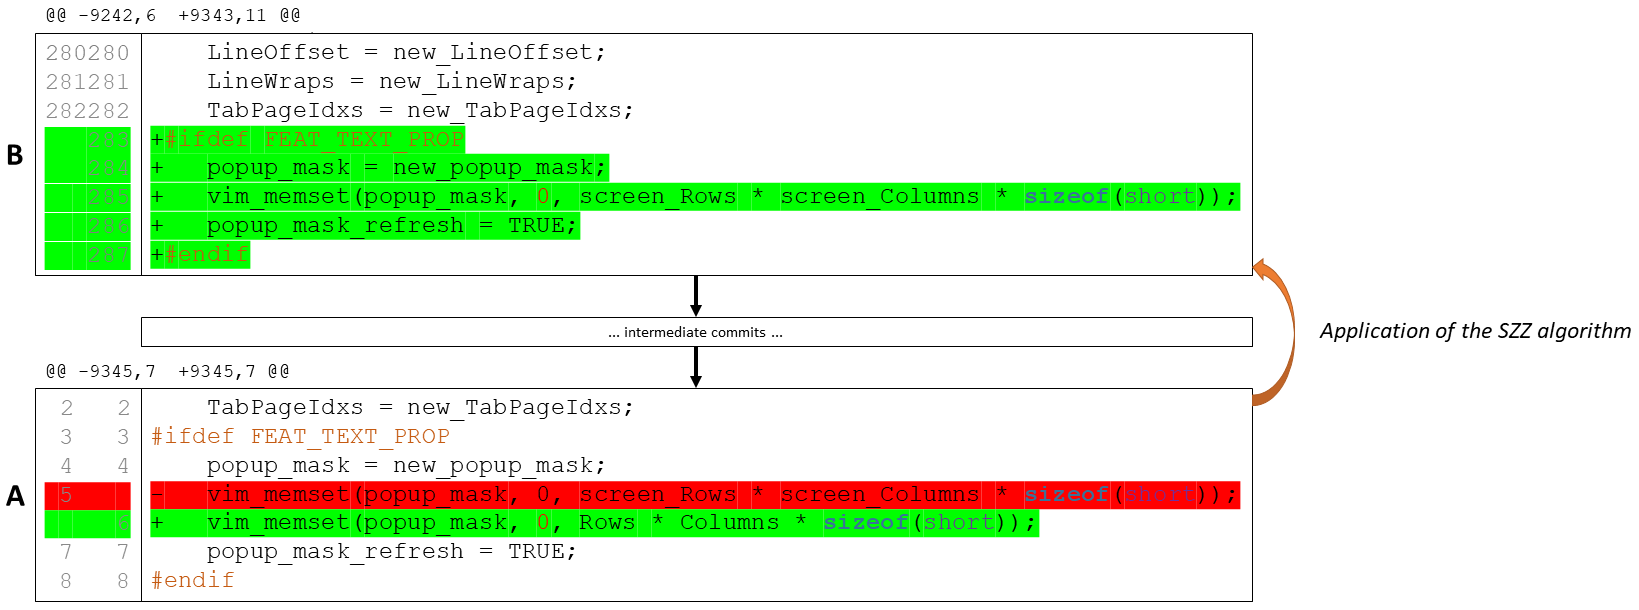
\includegraphics[width=\textwidth]{Bug_example_real}
    \Description{Real example of a defect.}
    \caption{Real example of a defect with corrective (A) and bug-introducing (B) commit\label{fig:bug-example}}
\end{figure*}


\subsection{Selection of Metrics}

As already mentioned, attributes are used to train the machine learning classifiers. In this scenario, so-called metrics are used as attributes. Metrics are numerical values that quantify properties of a software project. In this case, the metrics are divided into the usual categories code metrics and process metrics and each is calculated using the existing raw data of the main tables \cite{Rahman2013}. Code metrics are used to measure properties of source code, such as "size" or complexity \cite{Rahman2013}. Process metrics are used to measure properties that can be discussed using metadata from software repositories \cite{Rahman2013}. Examples include the number of changes made to a particular file or the number of active developers on a project. For this work, eleven feature-based metrics were calculated, divided into seven process and four code metrics. Five of the process metrics were taken from scientific papers \cite{Rahman2013,Queiroz2016}. The other six metrics were calculated based on the commit metadata obtained from PyDriller. A list of the eleven metrics and their descriptions can be found in \autoref{tab:metrics}. The individual metrics were calculated either directly using SQL queries or combined using SQL queries and calculations by a Python script.

In view of the evaluation of the feature-based dataset that follows in the next section, two additional datasets were created to make the impact of the feature-based metrics on the classifiers' predictions comparable. Both further data sets follow a classical file-based approach as it is common in machine learning based error detection and are based on the methodology developed by Moser et al. \cite{Moser2008}. The 17 process metrics of this scientific work were also adopted and are listed in \autoref{tab:metrics-moser}. A visualization to distinguish the three data sets is shown in \autoref{fig:dataset}.

\begin{table*}[ht]
\centering
\caption{Overview of used feature-based metrics}
\label{tab:metrics}
\resizebox{\linewidth}{!}{%
\begin{tabular}{|>{\hspace{0pt}}p{0.027\linewidth}|>{\hspace{0pt}}p{0.318\linewidth}|>{\hspace{0pt}}p{0.584\linewidth}|>{\centering\arraybackslash\hspace{0pt}}p{0.064\linewidth}|} 
\cline{2-4}
\multicolumn{1}{>{\hspace{0pt}}p{0.027\linewidth}|}{}  & \textbf{Metric}                            & \textbf{Description}                                                                                                                                                                                                                                               & \textbf{Source}   \\ 
\hline
\multirow{7}{0.027\linewidth}{\hspace{0pt}\rotatebox[origin=c]{90}{Process metrics}\textbf{}} & Number of commits                          & number of commits associated with the feature in a release.                                                                                                                                                                                                        & \cite{Queiroz2016,Rahman2013}              \\ 
\cline{2-4}
                                                       & Number of active developers                & number of developers who have edited (changed, deleted or added) \par{}the feature within a release.                                                                                                                                                               & \cite{Queiroz2016,Rahman2013}              \\ 
\cline{2-4}
                                                       & Number of distinct developers              & cumultative number of developers who have edited (changed, deleted or added) \par{}the feature within a release.                                                                                                                                                   & \cite{Queiroz2016,Rahman2013}              \\ 
\cline{2-4}
                                                       & Experience of all develepoers              & geometric mean of the experience of all developers who have edited \par{}(changed, deleted or added) the feature within a release. Experience is\par{}defined as the sum of the changed, deleted or added \par{}lines in the commits associated with the feature.  & \cite{Queiroz2016,Rahman2013}              \\ 
\cline{2-4}
                                                       & Experience of the most involved developers & experience of the developer who has edited (changed, deleted or added) \par{}the feature most often within a release. Experience is defined as the \par{}sum of changed, deleted, or added lines in the commits associated with the \par{}feature.                 & \cite{Queiroz2016,Rahman2013}              \\ 
\cline{2-4}
                                                       & Degree of modifications                    & number of edits (change, removal, extension) of the feature within a release.                                                                                                                                                                                      & *                 \\ 
\cline{2-4}
                                                       & Scope of modifications                     & number of edited features within a release (feature overlapping value). \par{}Idea: The more features have been edited in a release, \par{}the more error-prone they seem to be.                                                                                   & *                 \\ 
\hline
\multirow{4}{0.027\linewidth}{\hspace{0pt}\rotatebox[origin=c]{90}{Code metrics}\textbf{}} & Lines of code                              & average number of lines of code of the files associated with the feature\par{}within a release.                                                                                                                                                                    & *                 \\ 
\cline{2-4}
                                                       & Cyclomatic Complexity                      & average cyclomatic complexity of the files associated with the feature\par{}within a release.                                                                                                                                                                      & *                 \\ 
\cline{2-4}
                                                       & Number of added lines                      & average number of lines of code added to the files associated with \par{}the feature within a release.                                                                                                                                                             & *                 \\ 
\cline{2-4}
                                                       & Number of removed lines                    & average number of lines of code deleted from the files associated \par{}with the feature within a release.                                                                                                                                                         & *                 \\ 
\hline
\multicolumn{4}{|>{\centering\arraybackslash\hspace{0pt}}p{0.993\linewidth}|}{\textit{* These values were calculated based on the metadata obtained with PyDriller.}\par{}\textit{Feature-level metrics were calculated based on the metadata of the underlying files.} }                                                                                                                    \\
\hline
\end{tabular}
}
\end{table*}

\begin{table*}[ht]
\centering
\caption{Feature metrics. To apply the metrics to a file, we aggregate the metric values of all features associated to the given file, using the listed aggregation operator.}
\label{tab:metrics}
\resizebox{\linewidth}{!}{%
\begin{tabular}{|l|l|l|l|c|} 
\cline{2-5}
\multicolumn{1}{l|}{}        & \textbf{Metric}                            & \textbf{Description}                                                                                                                                                                                                                                                                           & \textbf{Aggregation~operator} & \textbf{Source}   \\ 
\hline
\multirow{7}{*}{\rotatebox[origin=c]{90}{Process metrics}\textbf{}} & Number of commits (FCOMM)                         & number of commits associated with the feature in a release.                                                                                                                                                                                                                                    & Mean                          & \cite{Queiroz2016,Rahman2013}              \\ 
\cline{2-5}
                             & Number of active developers (FADEV)              & \begin{tabular}[c]{@{}l@{}}number of developers who have edited (changed, deleted or added) \\the feature within a release.\end{tabular}                                                                                                                                                       & Mean                          & \cite{Queiroz2016,Rahman2013}              \\ 
\cline{2-5}
                             & Number of distinct developers (FDDEV)              & \begin{tabular}[c]{@{}l@{}}cumultative number of developers who have edited (changed, deleted or added) \\the feature within a release.\end{tabular}                                                                                                                                           & Mean                          & \cite{Queiroz2016,Rahman2013}              \\ 
\cline{2-5}
                             & Experience of all develepoers (FEXP)             & \begin{tabular}[c]{@{}l@{}}geometric mean of the experience of all developers who have edited \\(changed, deleted or added) the feature within a release. Experience is\\defined as the sum of the changed, deleted or added \\lines in the commits associated with the feature. \end{tabular} & Mean                          & \cite{Queiroz2016,Rahman2013}              \\ 
\cline{2-5}
                             & Experience of the most involved developers (FOEXP) & \begin{tabular}[c]{@{}l@{}}experience of the developer who has edited (changed, deleted or added) \\the feature most often within a release. Experience is defined as the \\sum of changed, deleted, or added lines in the commits associated with the \\feature. \end{tabular}                & Mean                          & \cite{Queiroz2016,Rahman2013}              \\ 
\cline{2-5}
                             & Degree of modifications (FMODD)                    & number of edits (change, removal, extension) of the feature within a release.                                                                                                                                                                                                                  & Mean                          & *                 \\ 
\cline{2-5}
                             & Scope of modifications (FMODS)                    & \begin{tabular}[c]{@{}l@{}}number of edited features within a release (feature overlapping value). \\Idea: The more features have been edited in a release, \\the more error-prone they seem to be. \end{tabular}                                                                              & Mean                          & *                 \\ 
\hline
\multirow{4}{*}{\rotatebox[origin=c]{90}{Code metrics}\textbf{}} & Lines of code (FNLOC)                              & \begin{tabular}[c]{@{}l@{}}average number of lines of code of the files associated with the feature\\within a release. \end{tabular}                                                                                                                                                           & Mean                          & *                 \\ 
\cline{2-5}
                             & Cyclomatic Complexity (FCyCO)                     & \begin{tabular}[c]{@{}l@{}}average cyclomatic complexity of the files associated with the feature\\within a release. \end{tabular}                                                                                                                                                             & Mean                          & *                 \\ 
\cline{2-5}
                             & Number of added lines (FADDL)                      & \begin{tabular}[c]{@{}l@{}}average number of lines of code added to the files associated with \\the feature within a release. \end{tabular}                                                                                                                                                    & Mean                          & *                 \\ 
\cline{2-5}
                             & Number of removed lines (FREML)                   & \begin{tabular}[c]{@{}l@{}}average number of lines of code deleted from the files associated \\with the feature within a release.\end{tabular}                                                                                                                                                 & Mean                          & *                 \\ 
\hline
\multicolumn{5}{|c|}{\begin{tabular}[c]{@{}c@{}}\textit{* These values were calculated based on the metadata obtained with PyDriller.}\\\textit{Feature-level metrics were calculated based on the metadata of the underlying files.} \end{tabular}}                                                                                                                                                                           \\
\hline
\end{tabular}
}
\end{table*}

\begin{table}
\centering
\caption{Process metrics according to \cite{Moser2008}}
\label{tab:metrics-moser}
\resizebox{\linewidth}{!}{%
\begin{tabular}{|l|l|} 
\hline
\textbf{Metric}   & \textbf{Description}                                                      \\ 
\hline
REVISIONS         & Number of revisions of a file.                                            \\ 
\hline
REFACTORINGS      & Number of times a file has been refactored.                               \\ 
\hline
BUGFIXES          & Number of times a file was involved in bug-fixing.                        \\ 
\hline
AUTHORS           & Number of distinct authors that checked a file into the repository.       \\ 
\hline
LOC\_ADDED        & Sum over all revisions of the lines of code added to a file.              \\ 
\hline
MAX\_LOC\_ADDED   & Maximum number of lines of code added for all revisions.                  \\ 
\hline
AVE\_LOC\_ADDED   & Average lines of code added per revision.                                 \\ 
\hline
LOC\_DELETED      & Sum over all revisions of the lines of code deleted from a file.          \\ 
\hline
MAX\_LOC\_DELETED & Maximum number of lines of code deleted for all revisions.                \\ 
\hline
AVE\_LOC\_DELETED & Average lines of code deleted per revision.                               \\ 
\hline
CODECHURN         & Sum of (added lines of code – deleted lines of code) over all revisions.  \\ 
\hline
MAX\_CODECHURN    & Maximum CODECHURN for all revisions.                                      \\ 
\hline
AVE\_CODECHURN    & Average CODECHURN per revision.                                           \\ 
\hline
MAX\_CHANGESET    & Maximum number of files committed together to the repository.             \\ 
\hline
AVE\_CHANGESET    & Average number of files committed together to the repository.             \\ 
\hline
AGE               & Age of a file in weeks (counting backwards from a specific release).      \\ 
\hline
WEIGHTED\_AGE     & $Weighted Age = \frac{\sum_{i=1}^N Age(i)*LOC\_ADDED(i)}{\sum_{i=1}^N LOC\_ADDED(i)}$                                                                    \\
\hline
\end{tabular}
}
\end{table}

\begin{figure*}[ht]
    \centering
    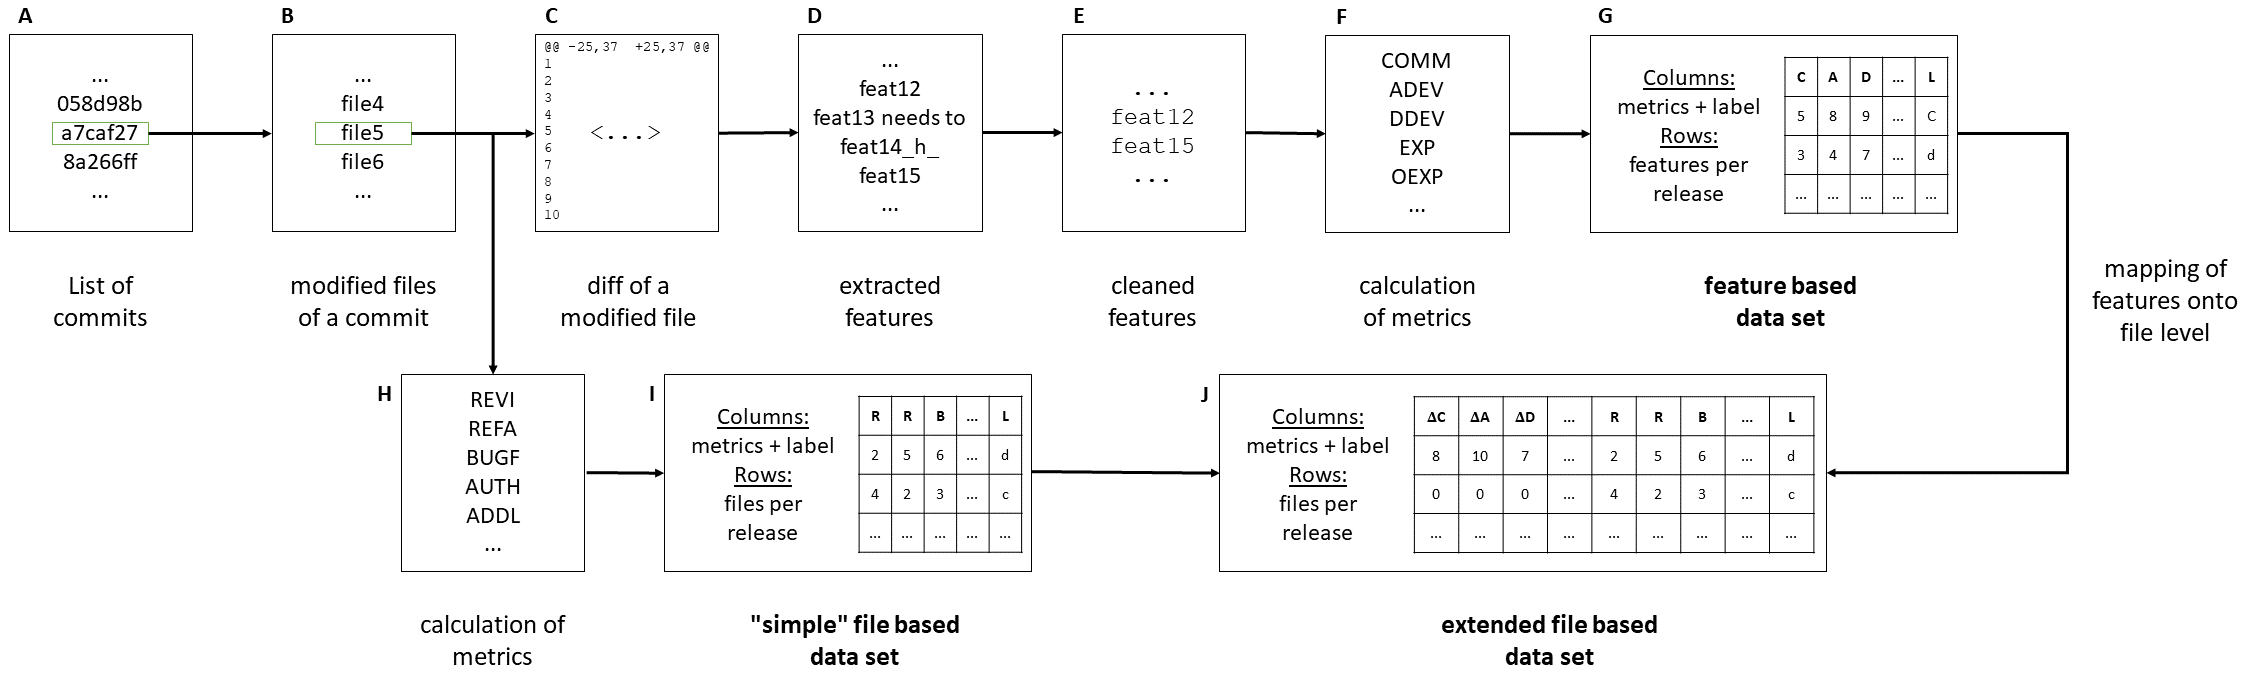
\includegraphics[width=\textwidth]{Dataset}
    \Description{Visualization to distinguish the three data sets.}
    \caption{Visualization to distinguish the three data sets\label{fig:dataset}}
\end{figure*}

The figure shows the ways of creating the feature-based dataset (path A - G) and the file-based data sets according  to \cite{Moser2008}.These are divided into the "simple" file-based dataset (paths A, B, H, I) and the extended file-based dataset (combination of both paths).  The creation of the feature-based dataset has already been explained in detail up to this section. More information about finalizing the datasets will follow as this section progresses.

The creation of the file-based datasets is also based on the raw data of the software project commits obtained with PyDriller and the modified files (A + B) extracted from them. Thus no further processing of the raw data is necessary. They then serve as a basis for the calculation of the 17 metrics (H) according to \cite{Moser2008}. To calculate the time-based metrics \texttt{AAGE} and \texttt{WAGE}, the raw data or the commits listed in the raw data had to be supplemented with their publication date. This was also done with PyDriller. The date of the first commit of a release was chosen as the starting point for calculating the past weeks.

The feature-based and the "simple" file-based dataset (G + I) consist of the calculated feature- (F) and file-related (H) metrics and the labels of the target class. The values of the metrics are calculated for the data of each software project. The resulting tables contain as columns the values of the eleven or 17 metrics and the label (target class) "defective" or "clean" and as rows the features or files aggregated by release.  This means that if a feature or file has been edited multiple times in a release (i.e. it is edited in multiple commits), the average value of the respective metrics within the release is calculated and stored. The procedure for determining the label is performed for each change to a feature or file using the following pattern:

\begin{table}[H]
\centering
\resizebox{\linewidth}{!}{%
\begin{tabular}{>{\hspace{0pt}}p{0.428\linewidth}>{\hspace{0pt}}p{0.046\linewidth}>{\hspace{0pt}}p{0.283\linewidth}>{\hspace{0pt}}p{0.046\linewidth}>{\hspace{0pt}}p{0.187\linewidth}}
bug-introducing       & + & corrective       & = & defective      \\
bug-introducing       & + & not corrective & = & defective      \\
not bug-introducing & + & corrective       & = & clean  \\
not bug-introducing & + & not corrective & = & clean 
\end{tabular}
}
\end{table}

The information on the status of a feature is based on the files on which it is based. If a feature or a file has been edited several times within a release, the label is determined according to the following rules:

\begin{itemize}
\setlength{\itemsep}{-2pt}
\item in the case of features, it is checked whether the feature was marked as "defective" at least once within the release. If this is the case, it is assumed that the feature is broken in the release in question. If this is not the case, the feature is assumed to be clean.
\item in the case of files, the last commit of the files in that release is checked. If the file is marked "clean" there, it is assumed to be error-free. If it is marked as "defective", it is assumed that it is defective in this release.
\end{itemize}

The individual tables created in this way are then concatenated into a common table, resulting in a comprehensive listing of metrics including the associated labels. This list specifies the characteristics a feature or file must have in order to be classified as "defective" or "clean" and serves as a training basis for classifiers for future predictions.

A special case is the second file-based data set created for the comparison within the evaluation (J). It is based on the "simple" file-based dataset (I) with the metrics from \cite{Moser2008}, but additionally includes the eleven metrics of the feature-based dataset (G) from \autoref{tab:metrics}. For this purpose, the values of the feature-based metrics were mapped or transferred at file level. This means that for each file of a release referenced in the file-based dataset, it was analyzed which features were mentioned in the respective file. From these features, the corresponding metrics of the feature-based dataset were determined and the average value was calculated and entered into the entered dataset. If no features were mentioned in a file, the value $0$ is stored for the feature-based metrics. As mentioned at the beginning of this section, this way the feature-based dataset can be compared with a classical file-based dataset, because the conditions for the comparison have been created. A direct comparison between the different datasets is not practical for the reasons mentioned above.

Some supplementary key figures for the datasets are listed in \autoref{tab:dataset-numbers}. The row "unique" indicates how many unique rows are contained in the datasets. The datasets created in the manner described above can now be used to train the classifiers. This process will be explained in the next section.

\begin{table}[ht]
\centering
\caption{Key figures of the data sets}
\label{tab:dataset-numbers}
\resizebox{\linewidth}{!}{%
\begin{tabular}{|l|r|r|r|} 
\hline
                     & \begin{tabular}[c]{@{}r@{}}\textbf{feature-based}\\\textbf{data set}\end{tabular} & \begin{tabular}[c]{@{}r@{}}\textbf{"simple" file-}\\\textbf{based data set}\end{tabular} & \begin{tabular}[c]{@{}r@{}}\textbf{"extended" file-}\\\textbf{based data set}\end{tabular}  \\ 
\hline
\#attributes         & $11$ + label                                                                        & $17$ + label                                                                               & $28$ + label                                                                                  \\ 
\hline
\#data records       & $14.059$                                                                            & $76.986$                                                                                   & $76.986$                                                                                      \\ 
\hline
~ ~thereof defective & $2.735$                                                                             & $1.899$                                                                                    & $1.899$                                                                                       \\ 
\hline
~ ~thereof clean     & $11.324$                                                                            & $75.087$                                                                                   & $75.087$                                                                                      \\ 
\hline
~ ~thereof unique    & $8.447$                                                                             & $52.564$                                                                                   & $52.783$                                                                                      \\
\hline
\end{tabular}
}
\end{table}

\subsection{Selection of Classifiers}

Although programming with the Python programming language was often used to create the data sets, the choice of a machine learning tool was not the library scikit-learn \cite{scikit}, but an independent solution. The WEKA-Workbench\footnote{\href{https://www.cs.waikato.ac.nz/ml/weka/}{https://www.cs.waikato.ac.nz/ml/weka/}} is used as a machine learning tool. This tool proved to be suitable for the underlying task by numerous citations in scientific papers (among others in \cite{Hammouri2018,Queiroz2016,Ratzinger2008}). The WEKA-Workbench (WEKA as acronym for \textbf{W}aikato \textbf{E}nvironment for \textbf{K}nowledge \textbf{A}nalysis) was developed at the University of Waikato in New Zealand and offers a large collection of machine learning algorithms and preprocessing tools for use within a graphical user interface \cite{Weka2016}. There are also interfaces for the Java programming language \cite{Weka2016}. An overview of the selected classification algorithms can be found in \autoref{tab:classifiers}. This also includes the abbreviations of the classifiers that will be used in the following.

\begin{table*}[ht]
\centering
\caption{Selection of classification algorithms}
\label{tab:classifiers}
\begin{tabular}{|l|l|} 
\hline
 \textbf{Algorithm}         & \textbf{Abbreviation}   \\ 
\hline
J48 Decision Trees          & J48                     \\ 
\hline
k-Nearest-Neighbors         & KNN                     \\ 
\hline
Logistic Regression         & LR                      \\ 
\hline
Na\"{\i}ve Bayes                  & NB                      \\ 
\hline
Artificial Neural Networks  & NN                      \\ 
\hline
Random Forest               & RF                      \\ 
\hline
Stochastic Gradient Descent & SGD                     \\ 
\hline
Support Vector Machines     & SVM                     \\
\hline
\end{tabular}
\end{table*}

All classification algorithms presented above are already integrated in the WEKA tool. It receives as input the final data sets in a proprietary file format. The 13 calculated metrics form the attributes, whereas the target class is represented by the labels "defective" and "clean".

The training process of the classifiers took place within the graphical user interface of WEKA. Before the training, the split ratios for the division of the data sets into training data and test data were determined. It was determined individually for each of the software projects used and is based on the number of releases available in each case. However, care was always taken to approximate the commonly used split ratios of 80:20 and 75:25 as well as $70:30$. The training data ranges from $67\%$ to $80\%$ of the data records of the data sets. The earlier releases were assigned to the training data. The training data contains the data records of the later releases. An overview of the division into training and test data per software project is shown in \autoref{fig:splits}. The resulting split ratios for the entire data sets are: $69:31$ (feature-based data set) and $71:29$ ("simple" and extended file-based data set).

\begin{figure*}[ht]
  \centering
  \subfloat[][Blender\\split ratio: $73:27$]{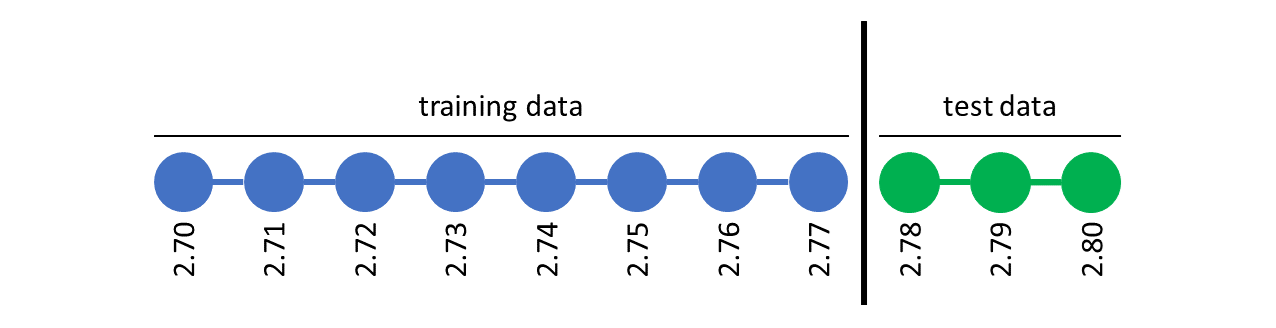
\includegraphics[width=0.5\linewidth]{release_blender}}
  \subfloat[][Busybox\\split ratio: $71:29$]{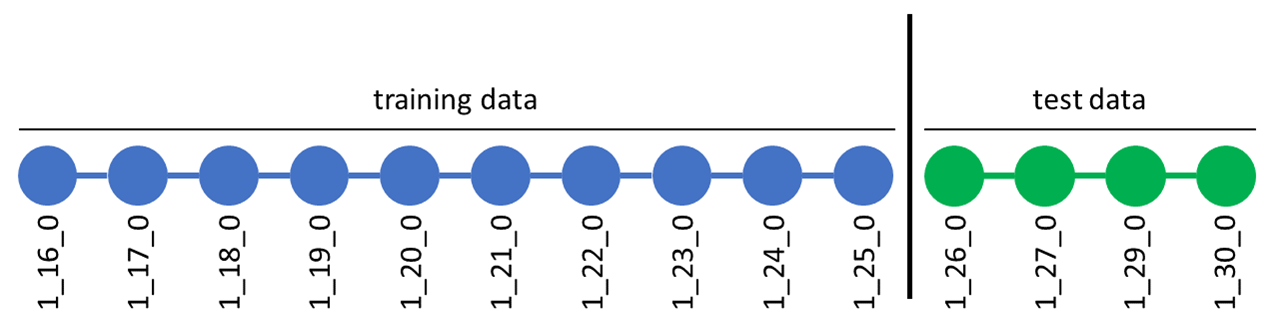
\includegraphics[width=0.5\linewidth]{release_busybox}}
  \qquad
  \subfloat[][Emacs\\split ratio: $71:29$]{
\includegraphics[width=0.5\linewidth]{release_emacs}}
  \subfloat[][GIMP\\split ratio: $71:29$]{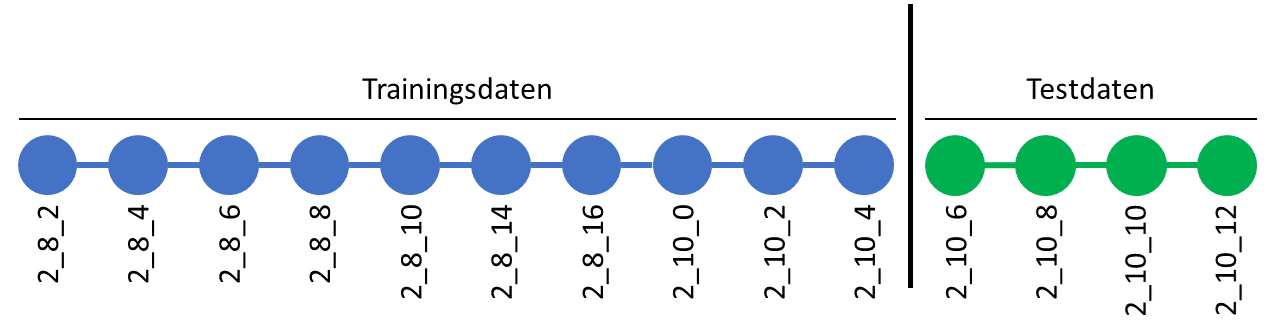
\includegraphics[width=0.5\linewidth]{release_gimp}}
  \qquad
  \subfloat[][Gnumeric\\split ratio: $75:25$]{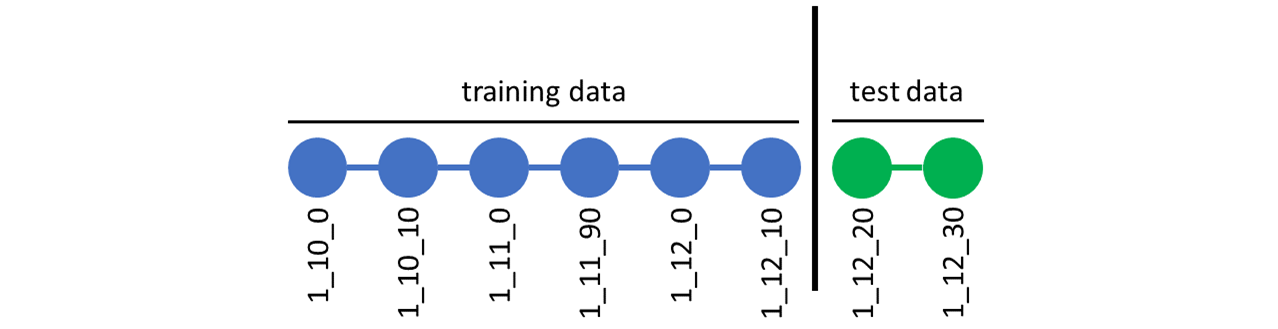
\includegraphics[width=0.5\linewidth]{release_gnumeric}}  
  \subfloat[][gnuplot\\split ratio: $80:20$]{
\includegraphics[width=0.5\linewidth]{release_gnuplot}}
  \qquad
  \subfloat[][Irssi\\split ratio: $71:29$]{
\includegraphics[width=0.5\linewidth]{release_irssi}}
  \subfloat[][libxml2\\split ratio: $80:20$]{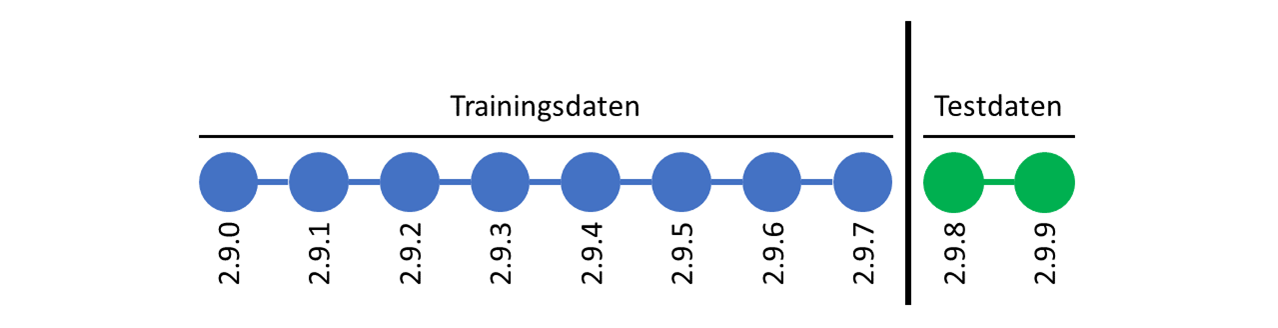
\includegraphics[width=0.5\linewidth]{release_libxml2}}
  \qquad
  \subfloat[][lighttpd\\split ratio: $67:33$]{
\includegraphics[width=0.5\linewidth]{release_lighttpd}}
  \subfloat[][MPSolve\\split ratio: $75:25$]{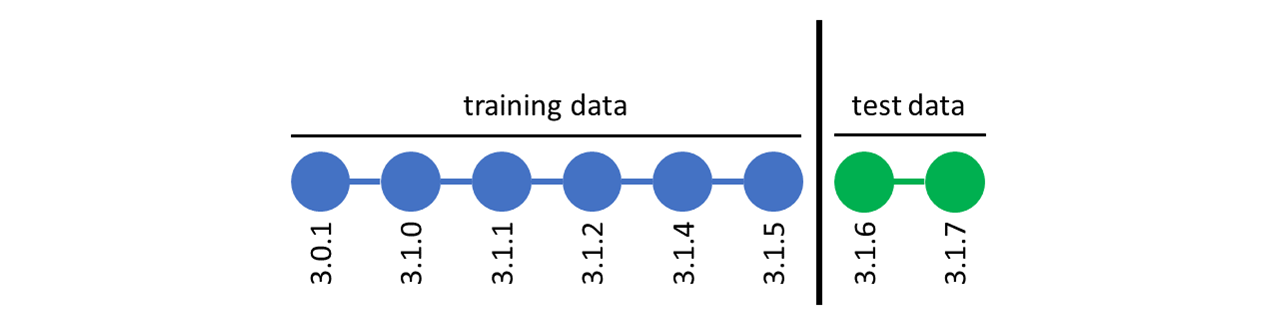
\includegraphics[width=0.5\linewidth]{release_mpsolve}}
  \qquad
  \subfloat[][Parrot\\split ratio: $71:29$]{
\includegraphics[width=0.5\linewidth]{release_parrot}}
  \subfloat[][Vim\\split ratio: $71:29$]{
\includegraphics[width=0.5\linewidth]{release_vim}}
  \Description{Overview of the division into training and test data.}
  \caption{Overview of the division into training and test data\label{fig:splits}}
\end{figure*}

The training of the classifiers in WEKA was carried out for each classification algorithm with the respective standard settings. Only for the algorithms NN and RF further configurations were made. For the RF-algorithm a number of instances of $200$ was defined. This means that 200 decision trees perform parallel processing at the same time. There are no clear recommendations on how many instances should be selected. The selected value of $200$ was therefore determined independently, taking into account the scope of the data sets and the high number of attributes. For the NN algorithm an independently determined hidden layer structure of \texttt{(13,13,13} was chosen. This means that the artificial neural network has three hidden layer layers of 13 hidden layer neurons each. This allows them to process the large number of attributes more efficiently. Furthermore, no validation data was generated, since it is not intended to perform attribute selection or to adjust further classifier settings.

An analysis of the training process also showed that the file-based data sets are highly unbalanced with regard to the target class. With a value of about $97\%$, there are far more entries assigned to the label "clean". Balancedness, i.e. a balanced ratio ($50:50$ is not mandatory in the binary case) within the target classes, is however a prerequisite for the correct training of most classifiers. Ignoring this problem can lead to misleading accuracy, since most records are correctly assigned to the over-represented class and is a fundamental problem of accuracy metrics. To solve this problem, the SMOTE algorithm was applied to the file-based datasets \cite{Chawla2002}. The algorithm, whose acronym stands for \textbf{S}ynthetic \textbf{M}inority \textbf{O}ver-sampling \textbf{Te}chnique, performs an oversampling of the underrepresented class \cite{Chawla2002}. Using next-neighbor calculations based on the Euclidean distance between the attribute values of each dataset's datasets, new synthetic datasets are added (oversampling) so that the number of datasets of the relevant class increases \cite{Chawla2002}. In this case, the percentage of synthetic records generated is 2000, so for each existing record of the underrepresented class, 20 additional synthetic records are generated. Thus, the percentage of records with the label "defective" was increased to about $41\%$. At the same time the number of records grew by about $60\%$. The algorithm was only applied to the training data \cite{Chawla2002} . It is not intended to be applied to the test data so that the "ground truth" is not distorted or falsified. As a result, the metrics of the file-based datasets also changed. These are shown in \autoref{tab:dataset-numbers-new}.

\begin{table*}[ht]
\centering
\caption{Key figures of the data sets}
\label{tab:dataset-numbers-new}
\begin{tabular}{|l|r|r|r|r|} 
\hline
\multirow{2}{*}{}    & \multicolumn{2}{c|}{\textbf{"simple" data set}} & \multicolumn{2}{c|}{\textbf{extended data set}}  \\ 
\cline{2-5}
                     & \textbf{before} & \textbf{after}                & \textbf{before} & \textbf{after}                 \\ 
\hline
\#attributes         & $17$ + label      & $17$ + label                    & $28$ + label      & $28$ + label                     \\ 
\hline
\#data records       & $76.986$          & $111.706$                       & $76.986$          & $112.706$                        \\ 
\hline
~ ~thereof defective & $1.899$           & $37.619$                        & $1.899$           & $37.619$                         \\ 
\hline
~ ~thereof clean     & $75.087$          & $75.087$                        & $75.087$          & $75.087$                         \\ 
\hline
~ ~thereof unique    & $52.564$          & $86.155$                        & $52.783$          & $86.381$                         \\ 
\hline
overall split ratio  & $71:29$           & $81:19$                         & $71:29$           & $81:19$                          \\
\hline
\end{tabular}
\end{table*}

The results obtained using the test data, which reflect the performance of the individual classifiers, are presented in the following chapter as part of the evaluation.


\setlength{\tymin}{3.5cm}
\begin{table*}[!t]
	\fontsize{7}{7}\selectfont
	\centering
	\caption{Let $R$ be a release consisting of $q$ commits: $\mathnormal{R = \{c_{1}, c_{2}, . . . c_{q}}\}$, $F$ be the set of all $p$ files changed by commits in $R$: $\mathnormal{F = \{f_{1}, f_{2}, . . . f_{p}}\}$. For each file $f\in F$, let $T$ be the set of all $n$ features (in $f$) affected by changes in $R$: $\mathnormal{T = \{feat_{1}, feat_{2}, . . . feat_{n}}\}$ , and each feature $feat\in T$ has a set $A$ of $m$ files which implement it: $A\subseteq F$: $\mathnormal{A = \{featfile_{1}, featfile_{2}, . . . featfile_{m}}\}$ We define our feature based metric as follows for each file \mformula{f}:}
	%\vspace{-.2cm}
	\label{tbl:featuredefects}
	\begin{threeparttable}
		\fontfamily{ptm}\selectfont
		
		\begin{tabulary}{\textwidth}{p{1cm}p{5cm}p{5cm}p{5cm}}
			
			\toprule
			\theader{metric}&\theader{description}	&	\theader{equation}	&	\theader{supplementary eq.}	\\
			\midrule
			$FCOMM$\tnote{1} & Average number of commits associated to the changed features of a file within a release. & $\mathit{FCOMM_R\,(f)} = \mathnormal{\dfrac{1}{n}\sum_{i=1}^{n} comm(feat_i,A_i)}$ & $\mathnormal{comm(feat_i,A_i) = \sum_{j=1}^{m} comm(featfile_j) }$ \\
			$FADEV$\tnote{2} & Average number of developers who changed the features of a files within a release. & $\mathit{FADEV_R\,(f)} = \mathnormal{\dfrac{1}{n}\sum_{i=1}^{n} adev(feat_i,A_i)}$ & $\mathnormal{adev(feat_i,A_i) = \sum_{j=1}^{m} adev(featfile_j) }$ \\
			$FDDEV$\tnote{3} & Average cumulated number of developers who changed the features of a files within a release. & $\mathit{FDDEV_R\,(f)} = \mathnormal{\dfrac{1}{n}\sum_{i=1}^{n} ddev(feat_i,A_i)}$ & $\mathnormal{ddev(feat_i,A_i) = \sum_{j=1}^{m} ddev(featfile_j) }$ \\
			$FEXP$\tnote{4} & Average experience\mtnote{5} of all developers who changed the features of a file within a release. & $\mathit{FEXP_R\,(f)} = \mathnormal{\dfrac{1}{n}\sum_{i=1}^{n} exp(feat_i,A_i)}$ & $\mathnormal{exp(feat_i,A_i) = \sum_{j=1}^{m} exp(featfile_j) }$ \\
			$FOEXP$\tnote{6} & Average experience\mtnote{5} of the developer who changed the features of a file most often within a release. & $\mathit{FOEXP_R\,(f)} = \mathnormal{\dfrac{1}{n}\sum_{i=1}^{n} oexp(feat_i,A_i)}$ & $\mathnormal{oexp(feat_i,A_i) = \sum_{j=1}^{m} oexp(featfile_j) }$ \\
			$FMODD$\tnote{7} & Average number of changes to the features of a file within a release. & $\mathit{FMODD_R\,(f)} = \mathnormal{\dfrac{1}{n}\sum_{i=1}^{n} modd(feat_i,A_i)}$ & $\mathnormal{modd(feat_i,A_i) = \sum_{j=1}^{m} modd(featfile_j) }$ \\
			$FMODS$\tnote{8} & Average number of changed features of a file within a release. & $\mathit{FMODS_R\,(f)} = \mathnormal{\dfrac{1}{n}\sum_{i=1}^{n} mods(feat_i,A_i)}$ & $\mathnormal{mods(feat_i,A_i) = \sum_{j=1}^{m} mods(featfile_j) }$ \\
			$FNLOC$\tnote{9} & Average number of lines of code of the underlying files of the changed features of a file within a release. & $\mathit{FNLOC_R\,(f)} = \mathnormal{\dfrac{1}{n}\sum_{i=1}^{n} nloc(feat_i,A_i)}$ & $\mathnormal{nloc(feat_i,A_i) = \sum_{j=1}^{m} nloc(featfile_j) }$ \\
			$FCYCO$\tnote{10} & Average cyclomatic complexity of the underlying files of the changed features of a file within a release. & $\mathit{FCYCO_R\,(f)} = \mathnormal{\dfrac{1}{n}\sum_{i=1}^{n} cyco(feat_i,A_i)}$ & $\mathnormal{cyco(feat_i,A_i) = \sum_{j=1}^{m} nloc(featfile_j) }$ \\								
			$FADDL$\tnote{11} & Average number of lines of code added to the underlying files of the changed features of a file within a release. & $\mathit{FADDL_R\,(f)} = \mathnormal{\dfrac{1}{n}\sum_{i=1}^{n} addl(feat_i,A_i)}$ & $\mathnormal{addl(feat_i,A_i) = \sum_{j=1}^{m} addl(featfile_j) }$ \\
			$FREML$\tnote{12} & Average number of lines of code deleted from the underlying files of the changed features of a file within a release. & $\mathit{FREML_R\,(f)} = \mathnormal{\dfrac{1}{n}\sum_{i=1}^{n} reml(feat_i,A_i)}$ & $\mathnormal{reml(feat_i,A_i) = \sum_{j=1}^{m} reml(featfile_j) }$ \\						
			\bottomrule				
		\end{tabulary}
		\begin{tablenotes}[para]
			~\item[1] $comm(featfile_j)$ counts commits in which the file $featfile_j$ was changed.
			~\item[2] $adev(featfile_j)$ counts the developers who changed the file $featfile_j$.  
			~\item[3] $ddev(featfile_j)$ cumulates the counts of developers who changed the file over commits $featfile_j$.
			~\item[4] $exp(featfile_j)$ returns the geometric mean of the experience\mtnote{5} of all developers who changed the file $featfile_j$.
			~\item[5] Experience is defined as the sum of the changed, deleted or added lines in the commits associated with the files.
			~\item[6] $oexp(featfile_j)$ returns the experience\mtnote{5} of the developer who changed the file $featfile_j$ most often within a release.
			~\item[7] $modd(featfile_j)$ returns the number of changes to the file $featfile_j$.
			~\item[8] $mods(featfile_j)$  returns the number of changed files in the release of the file $featfile_j$.
			~\item[9] $nloc(featfile_j)$ returns the number of lines of code of the file $featfile_j$.
			~\item[10] $cyco(featfile_j)$ returns the cyclomatic complexity of the file $featfile_j$.
			~\item[11] $addl(featfile_j)$ returns the number of added lines of code to the file $featfile_j$.
			~\item[12] $reml(featfile_j)$ returns the number of removed lines of code from the file $featfile_j$.
		\end{tablenotes}
	\end{threeparttable}
	\vspace{-0.3cm}
	%	\tbottom
\end{table*}